% ============================================================
%  第五卷 第十五章 表面（§154–§163 + 习题）
%  底本：高教社中文版第5版（束仁贵/束莼 译，郑伟谋 校）
%  OCR 底稿 full_merged.md 行 17347–18042（§163 之后即索引，未排）
%  插图 4 幅：图77（§155）、图78（§160）、图79/图80（§161）
%  习题 2 题附于 §162 末（与原书一致）
%  正文圈码 ①②…（共 15 处）已全部还原为 \footnote，脚注文本按 pages300
%  页面逐页转录（页面分布：p459①、p461①②、p462①②、p464①、p467①、
%  p468①、p469①②、p470①、p471①、p474①②、p477①）；
%  §154/§157 两条脚注内含独立公式，按 ch05 先例用 equation* 排于 \footnote 内；
%  §155 脚注②（Ландау 1950 俄文文献）与 §159 脚注①（两段）照原书转录。
%
%  已修正的 OCR/原书错误（除注明外均对照 原书转换/pages/p-459…p-479.png 核验）：
%   [全章] 分界面面积符号 OCR 乱作 §、\hat{\varsigma}、\tilde{\varsigma}、
%         \mathcal{G}、β、3、\vec{\mathfrak{s}}、\vec{\diamond} 等十余种，
%         统一按原书花体 𝔰 排 \mathfrak{s}；
%         偏差记号 OCR 之 "SP/8P/𝔖P" 统一为 δP；
%   [§154] "热力学势 𝒂""势函数 Ω_Ω"按 p-445 为热力学势 Ω；
%         V_z→V₂、N_•→N_s、S_{∘2}→S_{s2}、E_{s2}∼E_{s1}→E_{s2}−E_{s1}；
%         "这个密度 α(−t)^{2−a}"按 p-446 为 ∝(−t)^{2−α}；
%   [§155] （虚边线为(1 6)）照原书 p-447（非 (1n̄)）；
%         (155.1) OCR "= 4 dx/dy"按 p-448 为"= 极小值"；(155.2) OCR 乱码
%         按 p-448 为 ∫z dxdy = 常数；
%         雅可比式方程右端原书即印 ∂(∂ζ/∂p, ∂f/∂q)/∂(p,q)（p-449），
%         按 (155.3) 乘 ∂(x,y)/∂(p,q) 之推导应为
%         ∂(∂ζ/∂p, ∂ζ/∂q)/∂(p,q)，系原书排印误，已改正；
%   [§156] (r∈fty)→(r→∞)；(156.6) 下标按原书括注"下标写成 l 和 g 以代替
%         1 和 2"（OCR 之 "1" 实为 l）排 δP_l、δP_g、v_l；
%         P_ν、P_B→P_g、P_∘→P₀；"对于液体中的气泡；"→"气泡，"；
%   [§157] (157.2) 行尾衍 \cdot 删；OCR "n_s a 和 (∂α/∂c)_i"按 p-452 为
%         "n_s 和 (∂α/∂c)_T"；微商下标 _{T,I}→_{T,P}；
%   [§158] (158.3) n_a→n_{as}（p-453 印 n_{as}）；(158.4) OCR "dw_a dx"之
%         衍 d 删；"x² 正比于"→ϰ²；(158.6) OCR "c{c_az_a²}"之衍 \c 删；
%   [§159] 点群 OCR 乱码按 p-455 为 C_n 和 C_nv；
%   [§160] μ_ν、μ_k→μ_g；"ρ 是液体的密度"前 OCR 乱码按 p-455 为 ρ；
%         "在相同的 μ′𝓕"按 p-457 为"在相同的 μ′ 下"；
%   [§162] (162.5)–(162.8) 诸式 "8P/8T"→δP/δT；"可得 q 形成核的概率"之
%         衍 q 删（p-460）；习题2 解之 φ→Φ（热力学势，全书体例）；
%   [§163] "(..,1950)"按 p-462 为（Л. Д. Ландау, 1950）；∂Φ/∂n 中 OCR
%         "π_n n/L + ψ"按 p-462 为 T ln(n/L) + ψ；
%   [习题] 习题2 之式(1)(2)为习题局部编号，按 ch12b 先例用 \tag{1}\tag{2}。
%
%  遗留问题：
%   - (156.6) 首项下标 scan 难辨 l/1，按紧随括注"下标写成 l 和 g"排 l；
%   - §160 "固气液面"一语系原书原貌（p-456），照排；
%   - §162 "取决小于还是大于临界的尺度"一语系原书原貌（p-459），照排；
%   - §155 "每个单位长度走 1/(na) 步台阶"系原书原貌（p-447），照排；
%   - §161 (161.3) 原书以非黑体斜体排 α₁₂+α₁₃+α₂₃=0，照排。
% ============================================================
\chapter{表面}

\section{表面张力}

到现在为止，我们一直忽略不同物体之间分界面的存在而引起的效应\footnote{实际上，相互接触的两相由一薄过渡层隔开；我们不关注其结构，可以把它看成是几何面.}.因为随着物体尺度（粒子数）的增加，表面效应比体积效应增强慢得多，所以在只研究物体的体性质时，忽略面效应完全合理.但是，有一系列现象却直接与分界面的性质有关.

分界面的热力学性质完全由如下定义的一个量（物体状态的函数）来表征.我们用 $\mathfrak{s}$ 表示分界面的面积，并考虑这个面积改变一个无限小量 $\mathrm{d}\mathfrak{s}$ 的可逆过程.在这个过程中所耗费的功显然正比于 $\mathrm{d}\mathfrak{s}$，也就是说，可以写成形式
\begin{equation}
  \mathrm{d}R=\alpha\,\mathrm{d}\mathfrak{s}.
\end{equation}
用这样方式确定的量 $\alpha$ 是分界面的基本特性，称为表面张力系数.

公式(154.1)与物体体积可逆变化时功的公式 $\mathrm{d}R=-P\mathrm{d}V$ 完全对应.因此可以说：$\alpha$ 对于表面所起的作用正如同压强之于体积.特别是，很容易证明：作用到分界面任何区域的边界围线单位长度上的力，其大小等于 $\alpha$，而方向沿围线的法线向内并与表面相切.

这里暗含 $\alpha$ 为正；以下将说明的确如此.假如 $\alpha<0$，那么作用到表面的边界围线上的力，其方向沿围线的法线向外，亦即会“拉伸”表面；换句话说，两相间的分界面会无限增大，亦即相将混合而根本不会存在.反之，当 $\alpha>0$ 时，分界面的面积倾向于取（在两相体积给定下的）最小可能值.因此举例来说，如果一个各向同性相浸没于另一相中，那么它取球状（当然，这里忽略了外场即重力场的作用）.

现在我们比较详细地来考虑同一纯物质的液体和蒸气这两个各向同性相之间分界面的表面张力.如果所考虑的是平衡中两相的分界面，则应当记住它们的压强和温度之间有确定的函数关系即相平衡曲线方程.同时，在本质上 $\alpha$ 只依赖于单自变量而不是二变量.

在不考虑表面效应的情形下，由（同一种物质的）两相所构成的系统，当整个系统的体积给定为 $V$ 时，其能量微分具有形式 $\mathrm{d}E=T\mathrm{d}S+\mu\mathrm{d}N$（在平衡时两相的温度 $T$ 和化学势 $\mu$ 都相等，因而可对整个系统直接写出这个等式）.当考虑到存在表面效应时，显然还必须把(154.1)式加到这个等式的右边：
\begin{equation}
  \mathrm{d}E=T\mathrm{d}S+\mu\mathrm{d}N+\alpha\,\mathrm{d}\mathfrak{s}.
\end{equation}
但是，不选能量而选择热力学势 $\Omega$ 即以 $T,\mu$（以及体积 $V$）为自变量的热力学势，则较为方便.这里用 $\Omega$ 的方便之处在于，$T$ 和 $\mu$ 在两相中有相同值（至于压强则在考虑表面效应以后一般不一致，参看§156）.势函数 $\Omega$ 的微分（仍在 $V$ = 常数下）是
\begin{equation}
  \mathrm{d}\Omega=-S\mathrm{d}T-N\mathrm{d}\mu+\alpha\,\mathrm{d}\mathfrak{s}.
\end{equation}
我们所考虑的系统的热力学量（例如 $E,\Omega,S$）可以表示成“体的”和“面的”两部分之和.但是这样的划分并不唯一，因为每一相中粒子数的确定只能精确到两相之间过渡层中粒子数的数量级；对于每一相的体积，也是一样.这种不确定程度正好与我们所感兴趣的表面效应同数量级.为使划分唯一，可以外加如下的自然条件：两相的体积 $V_1$ 和 $V_2$ 相加应有等式 $V_1+V_2=V$（式中 $V$ 是系统的总体积），并且还有等式
\begin{equation*}
  n_1V_1+n_2V_2=N,
\end{equation*}
式中 $N$ 是系统中的粒子总数，而 $n_1=n_1(\mu,T)$ 和 $n_2=n_2(\mu,T)$ 是每一相（当作无边界时）粒子数的体积密度.这两个等式确定了体积 $V_1,V_2$（以及粒子数 $N_1=n_1V_1,N_2=n_2V_2$）的选择，从而也确定了所有其它热力学量体积部分的值.我们用角标 0 记体积部分，而表面部分用角标 s 记；根据以上定义，有粒子数 $N_s=0$.

由(154.3)，在恒定的 $T$ 和 $\mu$（因而 $\alpha$ 恒定）下，有 $\mathrm{d}\Omega=\alpha\,\mathrm{d}\mathfrak{s}$；所以显然 $\Omega_s=\alpha\mathfrak{s}$.因此
\begin{equation}
  \Omega=\Omega_0+\alpha\mathfrak{s}.
\end{equation}
因为熵 $S=-\left(\dfrac{\partial\Omega}{\partial T}\right)_{\mu,\mathfrak{s}}$，所以它的表面部分为\footnote{平衡态的系数 $\alpha$ 是单自变量函数；这样的函数对 $\mu$ 和 $T$ 的偏导数，本身没有意义.但是，取了
\begin{equation*}
  N_s=-\left(\frac{\partial\Omega_s}{\partial\mu}\right)_T=0,
\end{equation*}
在形式上已令 $\left(\dfrac{\partial\alpha}{\partial\mu}\right)_T=0$；这时显然有
\begin{equation*}
  \frac{\mathrm{d}\alpha}{\mathrm{d}T}=\left(\frac{\partial\alpha}{\partial T}\right)_\mu,
\end{equation*}
这已用在(154.5)中.}
\begin{equation}
  S_s=-\frac{\partial\Omega_s}{\partial T}
  =-\mathfrak{s}\frac{\mathrm{d}\alpha}{\mathrm{d}T}.
\end{equation}
其次，我们来求表面自由能；因为 $F=\Omega+N\mu$，而 $N_s=0$，所以
\begin{equation}
  F_s=\alpha\mathfrak{s}.
\end{equation}
表面能为
\begin{equation}
  E_s=F_s+TS_s
  =\left(\alpha-T\frac{\mathrm{d}\alpha}{\mathrm{d}T}\right)\mathfrak{s}.
\end{equation}
在表面积从 $\mathfrak{s}_1$ 变到 $\mathfrak{s}_2$ 的可逆等温过程中，所吸收的热量等于
\begin{equation}
  Q=T(S_{s2}-S_{s1})
  =-T\frac{\mathrm{d}\alpha}{\mathrm{d}T}
  (\mathfrak{s}_2-\mathfrak{s}_1).
\end{equation}
在这个过程中，热量 $Q$ 和功 $R=\alpha(\mathfrak{s}_2-\mathfrak{s}_1)$ 之和等于能量的改变 $E_{s2}-E_{s1}$，理应如此.

对应态定律（§84）也可定性地应用于液体及其蒸气之间的表面张力.由临界温度和压强可构造一个量纲为 $\mathrm{erg/cm^2}$ 的量，根据对应态定律的精神可以预料，$\alpha$ 与这个量的无量纲比值将是约化温度 $T/T_c$ 的普适函数：
\begin{equation}
  \frac{\alpha}{(T_cP_c^2)^{1/3}}=f\left(\frac{T}{T_c}\right)
\end{equation}
（在温度远低于临界时，这个比值约等于4）.

在临界点，液相与气相变为等同，它们的界面不再存在，表面张力系数应该变为零.根据临界点涨落理论的概念，其趋于零的规律可以用§148中引入的临界指数描述.

趋近临界点时，两相之间的过渡层宽度增加，并达到宏观的线度.在离临界点足够近的地方，这个宽度应该是涨落关联半径 $r_c$ 的数量级.现在只需要把宽度乘上热力学势密度的特征量，更确切地说，是与临界现象有关的奇异部分，便可得出表面张力.这个密度 $\propto(-t)^{2-\alpha}$（参看(153.12)的脚注）\footnote{用同一个字母 $\alpha$ 标记表面张力与临界指数大概不致于引起误解.}.因此，表面张力系数 $\propto r_c(-t)^{2-\alpha}$；注意到，根据(148.6) $r_c\propto(-t)^{-\nu}$，根据(149.2) $2-\alpha=\nu d=3\nu$，最后，我们求得
\begin{equation}
  \alpha\propto(T_c-T)^{2\nu}
\end{equation}
（B. Widom, 1965）.事实上 $2\nu\approx1.3$\footnote{在范德瓦尔斯理论中，过渡层的厚度也等于关联半径，因而表面张力的规律 $\propto(-t)^{2-\alpha-\nu}$（未用到关系式(149.2)）在该理论中也成立.从 $\alpha=0,\ \nu=1/2$ 得到 $(-t)^{3/2}$.}.

\section{晶体表面的张力}

晶体作为各向异性的物体，在不同的面上表面张力不同；可以说，表面张力是界面方向（即米勒指数）的函数，我们阐明这种关系的特征.\footnote{详见：Ландау Л. Д. О равновесной форме кристаллов.//Сборник, посвященный семидесятилетию акад. А. Ф. Иоффе. —М.: Изд-во АН СССР, 1950. p.~44；Ландау Л. Д. // Собрание трудов. —М.: Наука, 1969. 第2卷，第70篇论文.}

为了简化讨论，我们考虑如图77所示正方网格形状的二维晶格.这时过晶格点的直线起晶面的作用.

\par\nopagebreak\noindent\begin{minipage}{\linewidth}\centering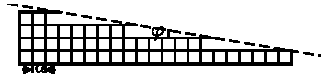
\includegraphics[width=7cm]{fig77.pdf}\\[0.3em]{\small 图 77}\end{minipage}\par\nopagebreak

设 $\alpha_0$ 是指数为$(01)$的面上的表面张力.我们考察与前者有小交角 $\varphi$ 的边线.它有指数$(1n)$且 n 很大.受边线限制的晶面，具有如图77所示的大宽度和给定高度的“阶梯”的形状.（虚边线为$(1\,6)$.）为明确起见，令高度等于晶格的周期 a. 这时每个单位长度走 $1/(na)$ 步台阶.每个台阶的存在导致出现某种附加的表面能量，我们用字母 $\beta$ 表示.当 n 很大时，每个台阶彼此相隔很远，相互作用可略.相对于表面张力 $\alpha_0$ 部分的附加项这时只不过由 $\beta$ 与单位长度所占台阶数的乘积即 $\beta/(na)$ 给出.

如果引入由边线$(1n)$与边线$(01)$所成角度 $\varphi$，则当 n 足够大时有 $\varphi\approx1/n$，因此边线$(1n)$的表面张力可以写成
\begin{equation*}
  \alpha=\alpha_0+\left(\frac{\beta}{a}\right)\varphi.
\end{equation*}
当 $\varphi$ 趋于 0（即 n 趋于无穷大）时，比值 $(\alpha-\alpha_0)/\varphi$ 因而趋于有限极限，它可以看成导数
\begin{equation*}
  \frac{\mathrm{d}\alpha}{\mathrm{d}\varphi}=\frac{\beta}{a}.
\end{equation*}
现在考虑指数为$(1\bar{n})$的边线，即具有负的 n 而相对于边线$(01)$反方向倾斜.由于现在台阶数为 $\dfrac{1}{|n|a}$，同样的讨论给出表面张力的变化量为 $\dfrac{\beta}{|n|a}$，因而
\begin{equation*}
  \alpha=\alpha_0-\frac{\beta}{a}\varphi,
\end{equation*}
并且导数等于
\begin{equation*}
  \frac{\mathrm{d}\alpha}{\mathrm{d}\varphi}=-\frac{\beta}{a}.
\end{equation*}
因此，表面张力是边界方向的非常特殊的函数.一方面，对于方向充分接近的两个晶面，其 $\alpha$ 值的差也充分小，即表面张力可以表示为面方向的连续函数的形式.另一方面，这个函数对每个 $\varphi$ 值在角度增加和减小的方向上分别有两个不同的导数值.

假定表面张力作为界面方向的函数已知.现在提出这样的问题：怎样借助于这个函数来确定晶体的平衡外形（刻面）；应当强调，在通常条件下所观察到的刻面决定于晶体的生长条件，而绝不是平衡外形.平衡外形决定于自由能 F 为极小值的条件（在给定的 T, N 和晶体体积 V 之下）或者等价地说自由能的表面部分.后者等于
\begin{equation*}
  F_s=\oint\alpha\,\mathrm{d}\mathfrak{s},
\end{equation*}
其中积分遍及晶体的整个表面（对于各向同性的物体，$\alpha$ = 常数，$F_s=\alpha\mathfrak{s}$，因而平衡外形直接决定于总面积 $\mathfrak{s}$ 为极小值的条件，亦即外形是球）.

设 $z=z(x,y)$ 是晶体表面的方程式，引入符号
\begin{equation*}
  p=\frac{\partial z}{\partial x},\qquad q=\frac{\partial z}{\partial y},
\end{equation*}
记决定表面在每一点的方向的两个微商；$\alpha$ 可以表示为它们的函数：$\alpha=\alpha(p,q)$. 平衡外形决定于条件
\begin{equation}
  \int\alpha(p,q)\sqrt{1+p^2+q^2}\,\mathrm{d}x\mathrm{d}y=\text{极小值},
\end{equation}
同时有附加条件
\begin{equation}
  \int z\,\mathrm{d}x\mathrm{d}y=\text{常数}
\end{equation}
（体积恒定）.这个变分问题导致微分方程
\begin{equation}
  \frac{\partial}{\partial x}\frac{\partial f}{\partial p}
  +\frac{\partial}{\partial y}\frac{\partial f}{\partial q}=2\lambda,
\end{equation}
式中引入了符号
\begin{equation}
  f(p,q)=\alpha(p,q)\sqrt{1+p^2+q^2},
\end{equation}
而 $\lambda$ = 常数.

其次，根据定义，我们有 $\mathrm{d}z=p\,\mathrm{d}x+q\,\mathrm{d}y$；引入辅助函数
\begin{equation}
  \zeta=px+qy-z,
\end{equation}
我们有 $\mathrm{d}\zeta=x\,\mathrm{d}p+y\,\mathrm{d}q$，即
\begin{equation}
  x=\frac{\partial\zeta}{\partial p},\qquad
  y=\frac{\partial\zeta}{\partial q},
\end{equation}
在这里 $\zeta$ 看成是 p 和 q 的函数.把(155.3)中对 x 和 y 的微商改写成雅可比式的形式，两边乘以 $\dfrac{\partial(x,y)}{\partial(p,q)}$，并利用(155.6)式，可得方程
\begin{equation*}
  \frac{\partial(\partial f/\partial p,\ \partial\zeta/\partial q)}{\partial(p,q)}
  +\frac{\partial(\partial\zeta/\partial p,\ \partial f/\partial q)}{\partial(p,q)}
  =2\lambda\frac{\partial(\partial\zeta/\partial p,\ \partial\zeta/\partial q)}{\partial(p,q)}.
\end{equation*}
这个方程有一个积分
\begin{equation*}
  f=\lambda\zeta=\lambda(px+qy-z),
\end{equation*}
即
\begin{equation}
  z=\frac{1}{\lambda}\left(p\frac{\partial f}{\partial p}
  +q\frac{\partial f}{\partial q}-f\right).
\end{equation}
此式不是别的，而就是如下平面族的包络面：
\begin{equation}
  px+qy-z=\frac{1}{\lambda}\alpha(p,q)\sqrt{1+p^2+q^2},
\end{equation}
式中 p, q 充当参数.

上面所得到的结果，可以用下述几何作图的形式来表述.在自坐标原点引出的每一根径矢上，截取一段长度正比于 $\alpha(p,q)$ 的线段，其中 p, q 决定径矢的方向\footnote{径矢的三个方向余弦正比于 $p,q,-1$.}.过线段端点作与之垂直的平面；则这些平面的包络给出晶体的外形.（G. V. Wulf, 1901）.

可以证明（参看本节第一个脚注所引文献）：由于在这一节开始时所提到的函数 $\alpha$ 的特殊性质，由这个定则所确定的晶体平衡外形，包含数个对应于小米勒指数晶面的平面区.这些平面区的大小随着米勒指数的增加而迅速减小.这实际上表明晶体的平衡外形由为数不多的平面区构成，它们不以显著的角度相交，而由圆滑区相联结.

\section{表面压强}

我们以两相作用在界面上的力相等为根据证明了（§12）相互接触的两相压强相等的条件.如同在别处，这里完全忽略了表面效应.显然，如果界面不是平面，则当它移动时，它的面积进而表面能一般也会发生变化.换句话说，两相之间有弯曲的界面存在，会导致出现附加力，结果两相的压强将不等；它们之差称为表面压强.

这个量取决于力学平衡条件：在界面处作用于每相的力的总和应该等于零.

我们考虑各向同性的两相（两种液体或液体和蒸气），假定其中一相（相1）是浸没在另一相中的球体.这时每一相内压强恒定.

现在保持系统总体积不变而使界面作无穷小可逆位移.根据§154开头所述，在此过程中所做的功可表示为
\begin{equation}
  \mathrm{d}R=-P_1\mathrm{d}V_1-P_2\mathrm{d}V_2+\alpha\,\mathrm{d}\mathfrak{s}
  =-(P_1-P_2)\mathrm{d}V_1+\alpha\,\mathrm{d}\mathfrak{s},
\end{equation}
式中指标 1 和 2 分别对应于两相.力学平衡条件为这个功等于零：
\begin{equation*}
  \mathrm{d}R=-(P_1-P_2)\mathrm{d}V_1+\alpha\,\mathrm{d}\mathfrak{s}=0.
\end{equation*}
最后，把 $V_1=\dfrac{4\pi}{3}r^3,\ \mathfrak{s}=4\pi r^2$（式中 r 是球的半径）代入这里，得到待求的公式
\begin{equation}
  P_1-P_2=\frac{2\alpha}{r}.
\end{equation}
在界面为平面的情形下（$r\to\infty$），两个压强相等，正如所料.

从力学平衡条件得到的公式(156.2)只定了两相压强之差.如果考虑同种物质的两相彼此之间处于完全的热力学平衡，这时可以分别计算每一相中的压强.实际上，压强 $P_1$ 和 $P_2$ 满足方程 $\mu_1(P_1,T)=\mu_2(P_2,T)$. 两相界面为平面时，其共同压强（用 $P_0$ 表示）在同样的温度下由关系式 $\mu_1(P_0,T)=\mu_2(P_0,T)$ 确定.两式逐项相减，有
\begin{equation}
  \mu_1(P_1,T)-\mu_1(P_0,T)=\mu_2(P_2,T)-\mu_2(P_0,T).
\end{equation}
假定偏差
\begin{equation*}
  \delta P_1=P_1-P_0,\qquad \delta P_2=P_2-P_0
\end{equation*}
相对的很小，将等式(156.3)的两边按它们展开，求得
\begin{equation}
  v_1\delta P_1=v_2\delta P_2,
\end{equation}
式中 $v_1,v_2$ 是两相的分子体积（参看(24.12)）.把公式(156.2)改写成 $\delta P_1-\delta P_2=2\alpha/r$，并与上式联立，得待求的 $\delta P_1$ 和 $\delta P_2$：
\begin{equation}
  \delta P_1=\frac{2\alpha}{r}\frac{v_2}{v_2-v_1},\qquad
  \delta P_2=\frac{2\alpha}{r}\frac{v_1}{v_2-v_1}.
\end{equation}
对于蒸气中的液滴，有 $v_1\ll v_2$；把蒸气看成理想气体，有 $v_2=T/P_2\approx T/P_0$，结果求得
\begin{equation}
  \delta P_l=\frac{2\alpha}{r},\qquad
  \delta P_g=\frac{2v_l\alpha}{rT}P_0
\end{equation}
（为明显起见，下标写成“l”和“g”以代替 1 和 2）.我们看到，液滴上的蒸气压随液滴半径的减小而增加，且超过平液面上的饱和蒸气压.

在液滴非常小的情形下，$\delta P_g/P_0$ 不再很小，公式(156.6)变得不适用，因为由于蒸气的体积强烈地依赖于压强，从(156.3)到(156.4)的展开不再允许.液体的压缩率很小，压强变化对其影响不大，方程(156.3)的左边仍可以用 $v_1\delta P_1$ 代替.把蒸气形为 $\mu=T\ln P_g+\chi(T)$ 的化学势代入右边，求得
\begin{equation*}
  \delta P_1=P_1-P_0=\frac{T}{v_1}\ln\frac{P_g}{P_0}.
\end{equation*}
因为在给定的情况下，$\delta P_1\gg\delta P_g$，所以差 $P_1-P_0$ 可用 $P_1-P_g$ 来代替，利用表面压强的公式(156.2)，最后我们得到
\begin{equation}
  \ln\frac{P_g}{P_0}=\frac{2\alpha v_1}{rT}.
\end{equation}
对于液体中的气泡，用类似的方式可以得出与(156.6)、(156.7)同样的公式，只是其中的符号正好相反.

\section{溶液的表面张力}

现在我们来考虑液态溶液和气相（任何气体及其在液体中的溶液、溶液及其蒸气等等）之间的界面.

像在§154中一样，我们把所考虑的系统的所有热力学量都划分为体积部分和表面部分；划分的方法由溶剂的体积和粒子数的条件 $V=V_1+V_2$ 和 $N=N_1+N_2$ 来决定.换句话说，系统的整个体积 V 全部划分到两相中去，因此，把 $V_1$ 和 $V_2$ 各乘以相应的溶剂粒子数的体积密度后，它们之和就正好等于系统中的溶剂粒子总数 N. 因此根据这个定义，表面部分 $N_s=0$.

像其它的量一样，溶质的粒子数也可以表示成两部分之和的形式：$n=n_0+n_s$.可以说，设想溶质在体积 $V_1$ 和 $V_2$ 中各以等于它在相应溶液中体积浓度值的恒定浓度分布，则 $n_0$ 是其中所含的总数.这样定义的粒子数 $n_0$ 可能大于，也可能小于溶质粒子的实际总数 n. 如果 $n_s=n-n_0>0$，那么这意味着溶质以较高的浓度积累在表面层中（称为正吸附）.如果 $n_s<0$，则表明在表面层中的浓度低于其体值（称为负吸附）.

溶液的表面张力系数不再只依赖于一个自变量，而是两个.因为热力学势 $\Omega$ 对化学势的微商（取反号）给出相应的粒子数，所以 $\Omega_s=\alpha\mathfrak{s}$ 对溶质的化学势 $\mu'$ 微分，可以得到 $n_s$\footnote{系数 $\alpha$ 现在是两个独立变量（例如 $\mu'$ 和 $T$）的函数；而微商 $\dfrac{\partial\Omega_s}{\partial\mu'}$ 应当在 $T$ 和溶剂的化学势 $\mu$ 都为恒定的条件下来取.但是我们所采纳的条件
\begin{equation*}
  N_s=-\left(\frac{\partial\Omega_s}{\partial\mu}\right)_{\mu',T}=0,
\end{equation*}
表明已形式地令 $\left(\dfrac{\partial\alpha}{\partial\mu}\right)_{\mu',T}=0$，因此可写等式(157.1)（参看§154第二个脚注).}：
\begin{equation}
  n_s=-\frac{\partial\Omega_s}{\partial\mu'}
  =-\mathfrak{s}\left(\frac{\partial\alpha}{\partial\mu'}\right)_T.
\end{equation}
我们假设：气相的压强是很小，以致于它对液相性质的影响可略.公式(157.1)中 $\alpha$ 的微商本应在给定温度下沿相平衡曲线来取，这里可以用在恒定（等于 0 的）压强（和恒定 T）下取的微商来代替.把 $\alpha$ 看作温度和溶液浓度 c 的函数，(157.1)式可改写成形式
\begin{equation}
  n_s=-\mathfrak{s}\left(\frac{\partial\alpha}{\partial c}\right)_T
  \left(\frac{\partial c}{\partial\mu'}\right)_{T,P}.
\end{equation}
但是根据热力学不等式(96.7)，微商 $\left(\dfrac{\partial\mu'}{\partial c}\right)_{T,P}$ 总是正的.因此由(157.2)得出：$n_s$ 和 $\left(\dfrac{\partial\alpha}{\partial c}\right)_T$ 具有相反的符号.这意味着：如果溶质的作用是提高表面张力（$\alpha$ 随着溶液浓度的增加而增大），那么有负吸附.然而，降低表面张力的物质则被正吸附.

如果溶液很稀，那么溶质的化学势具有 $\mu'=T\ln c+\psi(P,T)$ 的形式；将之代入(157.2)，得
\begin{equation}
  n_s=-\mathfrak{s}\frac{c}{T}\left(\frac{\partial\alpha}{\partial c}\right)_T.
\end{equation}
对于（压强 P 下）液体表面的气体吸附，可以得到类似的公式：
\begin{equation}
  n_s=-\mathfrak{s}\frac{P}{T}\left(\frac{\partial\alpha}{\partial P}\right)_T.
\end{equation}
如果不仅溶液很稀，而且溶液的吸附也很弱，那么 $\alpha$ 可按 c 的幂次展开成级数，并近似地写成：
\begin{equation*}
  \alpha=\alpha_0+\alpha_1 c,
\end{equation*}
式中 $\alpha_0$ 是纯溶剂两相界面的表面张力.于是由(157.3)我们求出：
\begin{equation*}
  \alpha_1=-\frac{n_s T}{\mathfrak{s}c},
\end{equation*}
因此
\begin{equation}
  \alpha-\alpha_0=-\frac{n_s T}{\mathfrak{s}}.
\end{equation}
值得指出，这个公式与渗透压的范霍夫公式在形式上相似（表面积在这里起体积的作用）.

\section{强电解质溶液的表面张力}

溶有强电解质时液体表面张力的改变，对于稀溶液可用普遍的方式计算（L. Onsager, N. Samaras, 1934）.

设离开自由面 x 处的离子（a 类）因自由面的存在而具有的附加能量为 $w_a(x)$（当 $x\to\infty$ 时，$w_a(x)$ 趋于零）.表面附近的离子浓度与溶液内部的浓度 $c_a$ 二者相差一个因子
\begin{equation*}
  \exp\left(-\frac{w_a}{T}\right)\approx1-\frac{w_a}{T}.
\end{equation*}
因此，表面对液体中这些离子总数的贡献为
\begin{equation}
  n_{as}=-\frac{\mathfrak{s}c_a}{vT}\int_0^{\infty}w_a\,\mathrm{d}x
\end{equation}
（v 是溶剂的分子体积）.

为了计算表面张力，我们从如下关系式出发
\begin{equation}
  \mathfrak{s}\,\mathrm{d}\alpha=-\sum_a n_{as}\,\mathrm{d}\mu'_a,
\end{equation}
式中求和对溶液中各类离子进行.对于稀溶液（$\mu'_a=T\ln c_a+\psi_a$）
\begin{equation}
  \mathfrak{s}\,\mathrm{d}\alpha=-T\sum_a\frac{n_{as}}{c_a}\,\mathrm{d}c_a.
\end{equation}
把(158.1)代入上式，得
\begin{equation}
  \mathrm{d}\alpha=\frac{1}{v}\sum_a\mathrm{d}c_a\int_0^{\infty}w_a\,\mathrm{d}x.
\end{equation}
稍后将会看到，积分的主要贡献来自比分子间距为大而又比德拜半径 $1/\varkappa$ 为小的距离 x\footnote{溶液中 $\varkappa^2$ 的表达式与(78.8)式的不同仅在于分母中的因子 $\varepsilon$.}.

能量 $w_a$ 由两部分构成：
\begin{equation}
  w_a=\frac{\varepsilon-1}{\varepsilon(\varepsilon+1)}
  \frac{e^2z_a^2}{4x}+ez_a\varphi(x).
\end{equation}
第一项来自所谓的“像力”，它施加在置于介电常数为 $\varepsilon$ 的介质中且与表面相距 x 的电荷 $ez_a$ 上.由于不等式 $x\ll1/\varkappa$，电荷 $ez_a$ 周围离子云的屏蔽效应并不影响这个能量.在第二项中，$\varphi(x)$ 代表溶液中所有其它离子所产生的势场由于表面的存在而发生的改变.但是这一项在这里并不重要，因为考虑到溶液的电中性（$\sum_a c_a z_a=0$，进而 $\sum_a z_a\,\mathrm{d}c_a=0$），将(158.5)代入(158.4)后这一项不再出现.

因此，(158.4)求积分后，得
\begin{equation*}
  \mathrm{d}\alpha=\frac{(\varepsilon-1)e^2}{4\varepsilon(\varepsilon+1)v}
  \sum_a\ln\frac{1}{\varkappa a_a}\,\mathrm{d}\bigl(z_a^2c_a\bigr).
\end{equation*}
积分在上、下限对数发散，证实了上述关于积分范围的说法.我们自然地取了屏蔽半径 $1/\varkappa$ 作为积分上限，而取原子线度量级的量 $a_a$（对于不同类型的离子有不同的值）作为积分下限.考虑到 $\varkappa^2$ 正比于 $\sum z_a^2c_a$，可以看出，所得到的表达式是一个全微分，因而可以直接积分，其结果为：
\begin{equation}
  \alpha-\alpha_0=\frac{(\varepsilon-1)e^2}{8\varepsilon(\varepsilon+1)v}
  \sum_a c_a z_a^2\ln\frac{\lambda_a z_a^2}{\sum_b c_b z_b^2},
\end{equation}
其中 $\alpha_0$ 是纯溶剂的表面张力，$\lambda_a$ 是无量纲常数.

这个式子解答了提出的问题.我们看到，溶入强电解质后液体的表面张力增大.

\section{吸附}

吸附在狭义下理解是指这种情形：溶质积聚在凝聚相（吸附剂）的表面\footnote{为了明确起见，这里考虑气相吸附.}，而几乎不透入其体积内.这样形成的吸附膜可以用“表面浓度”$\gamma$ 来表征，它定义为单位表面积上被吸附物质（吸附质）的粒子数.如果发生吸附的气体压强很小，浓度 $\gamma$ 应当与压强成正比\footnote{但是这个规则在固体表面吸附中实际上并不满足，因为事实上这种表面并非总是足够均匀.}；当压强很大时，$\gamma$ 的上升变慢，而趋于一个极限值，对应于吸附质分子紧密堆积形成单分子层.

设 $\mu'$ 是吸附质的化学势.用§96中对于体积溶液所用过的同样方法，对于吸附我们可以得到热力学不等式
\begin{equation}
  \left(\frac{\partial\mu'}{\partial\gamma}\right)_T>0,
\end{equation}
这与不等式(96.7)完全类似.另一方面，由(157.1)我们有：
\begin{equation}
  \gamma=-\left(\frac{\partial\alpha}{\partial\mu'}\right)_T
  =-\left(\frac{\partial\alpha}{\partial\gamma}\right)_T
  \left(\frac{\partial\gamma}{\partial\mu'}\right)_T,
\end{equation}
考虑到不等式(159.1)，由此得出：
\begin{equation}
  \left(\frac{\partial\alpha}{\partial\gamma}\right)_T<0,
\end{equation}
即表面张力随着表面浓度的增加而降低.

形成吸附膜所必须做的最小功，等于热力学势 $\Omega$ 相应的改变：
\begin{equation}
  R_{\mathrm{min}}=\mathfrak{s}(\alpha-\alpha_0),
\end{equation}
式中 $\alpha_0$ 是纯净表面上的表面张力.由此我们根据(91.4)求出吸附热
\begin{equation}
  Q=-\mathfrak{s}T^2\left(\frac{\partial}{\partial T}
  \frac{\alpha-\alpha_0}{T}\right)_P.
\end{equation}
吸附膜可以看成二维热力学系统，它可以是各向同性的，也可以是各向异性的，尽管两体积相是各向同性的\footnote{我们在这里考虑液体表面吸附；固体表面吸附对这里的讨论意思不大，因为上面已经提到，事实上固体表面几乎总是有不均匀性. 应当指出，在同一纯物质的各向同性的两相（液态和蒸气）之间出现关于各向异性的界面，原则上也是可能的.}.因此就发生关于吸附膜可能对称类型的问题.

在§137的末尾已经提到，虽然不可能存在线度任意大的二维晶格（由于热涨落的“抹平”），如果薄膜的尺寸相对有限，它仍然可以表现出固体晶态的性质.正如§138末尾所指出的，抹平的结构仍保持各向异性.这种各向异性膜的对称类型应当按照点群来分类.这时绕轴的转动和相对于平面的反映，当然应该使薄膜平面与自身重合而且使两相的相互位置也保持不变，薄膜就位于两相的界面上.后者意味着，对称面不可能与薄膜平面重合.因此，薄膜只可能具有垂直于它的平面的对称轴以及过这根轴的对称面.换句话说，薄膜可能的对称类型只限于点群 $C_n$ 和 $C_{nv}$.

与三维物体的情况一样，在二维薄膜中也可能存在不同的相.薄膜的两相平衡条件除了要求它们的温度和化学势相等以外，还要求它们的表面张力相等.这后一个条件相当于在体积相中的压强相等条件，并且只不过表示要求两相彼此作用的力应当平衡.

\section{润湿}

我们考虑吸附质的蒸气当压强接近于饱和压强时在固体表面上的吸附.平衡时的浓度 $\gamma$ 取决于等化学势条件：吸附质的化学势 $\mu'$ 与蒸气的 $\mu_g$ 相等.这时可能出现几种情形，视 $\mu'$ 依赖于 $\gamma$ 的特征而定.

假定吸附质的量逐渐增加，吸附层变为宏观厚的液体膜，表面浓度 $\gamma$ 在这时约定取正比于液膜厚度 l 的一个量：$\gamma=\rho l/m$，式中 m 是分子的质量，$\rho$ 是液体的密度.膜厚增加时，吸附质的化学势趋于液体化学势的体值 $\mu_1$.我们约定从这个极限值起计量 $\mu'$ 值（在给定的 P 和 T 下），即以后将 $\mu$ 写成 $\mu'+\mu_1$，因此，根据定义当 $\gamma\to\infty$ 时，$\mu'\to0$.

蒸气的化学势可以表示为
\begin{equation*}
  \mu_g=\mu_1(T)+T\ln\frac{P}{P_0},
\end{equation*}
式中 $P_0(T)$ 是饱和蒸气压；这里用到了饱和蒸气压的定义，它是与液体呈平衡之值，即当 $P=P_0$ 时应该有 $\mu_g=\mu_1$\footnote{我们把液体看成是不可压缩的，即忽略它的化学势与压强的依赖关系.}.表面的浓度取决于条件 $\mu'+\mu_1=\mu_g$，即
\begin{equation}
  \mu'(\gamma)=T\ln\frac{P}{P_0}.
\end{equation}
假定有几个 $\gamma$ 值满足该方程，则其中使得势 $\Omega_s$ 取极小值者对应于稳定态.考虑它的单位面积表面之值，我们得到可称作固气液面（任意层厚下）“有效表面张力系数”$\alpha$ 的一个量，它可反映界面层的存在.具体地说，把关系式(159.2)积分，可写
\begin{equation}
  \alpha(\gamma)=\int_{\gamma}^{\infty}\gamma
  \frac{\mathrm{d}\mu'}{\mathrm{d}\gamma}\,\mathrm{d}\gamma
  +\alpha_{sl}+\alpha_{lg}.
\end{equation}
常数的选取，应使得 $\gamma\to\infty$ 时函数 $\alpha(\gamma)$ 化为固-液和液-气体相界面的表面张力之和.

还应指出，不等式(159.1)在任何 $\gamma$ 下成立，是热力学态稳定性的必要条件.

现在我们考虑几种典型的情况，它们依据函数 $\mu'(\gamma)$ 的特征而出现.在以下的图78中，实线表示这个函数在宏观厚的液膜区内的形式，而虚线对应于“分子厚度”的吸附膜区.当然，这两区的函数用一种比例表示，严格地说是不可能的，在这个意义上，这些图有随意性.

在图示的第一种情况（图78a）下，在薄膜的宏观厚度范围内函数 $\mu'(\gamma)$ 随 $\gamma$（即随膜厚）的增长而单调减小.至于在分子线度区内，则在这里函数 $\mu'(\gamma)$ 当 $\gamma\to0$ 时总是按规律 $\mu'=T\ln\gamma$ 趋于 $-\infty$，这对应于吸附质在表面的“稀溶液”.根据(160.1)，平衡浓度取决于曲线与水平线 $\mu'=$ 常数 $\leqslant0$ 的交点.这里的情形下，这只发生在分子浓度区，即应该发生上节所述的通常分子吸附.

如果 $\mu'(\gamma)$ 是单调上升处处为负的函数（图78b），则平衡时在吸附剂表面形成宏观厚度的液膜.尤其是，当压强 $P=P_0$（饱和蒸气）时生成的膜应当很厚，以致于里面物质的性质已经与液态的体性质没有区别，结果饱和蒸气与自己的液相接触.在这种情形下，我们说液体完全润湿这里的固体表面.

原则上也可能有更复杂的情况.例如，如果函数 $\mu'(\gamma)$ 穿过零点且有极大值（图78c），则有润湿发生，但仅在厚度小于一定的极限值时形成稳定膜.与 A 点对应的有限厚度膜同饱和蒸气处于平衡.亚稳态区 AB 以及完全不稳定区 BC 将该状态与别的稳定态（固体壁与体性质液体的平衡态）隔开.

\par\nopagebreak\noindent\begin{minipage}{\linewidth}\centering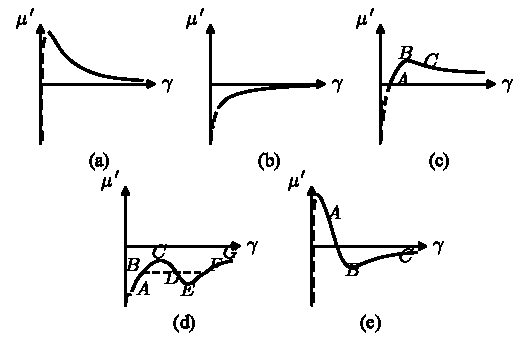
\includegraphics[width=11cm]{fig78.pdf}\\[0.3em]{\small 图 78}\end{minipage}\par\nopagebreak

如图78d所示类型的曲线对应于在一定厚度区内不稳定的薄膜.直线 BF 截得相等的面积 BCD 和 DEF，并联结 B 点和 F 点，这两点具有相同的 $\alpha$ 值（在相同的 $\mu'$ 下，这从(160.2)很容易看出）.分支 AB 和 FG 对应于稳定膜；区间 CE 完全不稳定，而区间 BC 和 EF 亚稳.

在这种情况下，不稳定区的两个边界（B 点和 F 点）对应于宏观膜厚.从某个宏观厚度到分子线度厚度的区间内的不稳定性似乎对应于图78e所示类型的曲线.然而，这种曲线更可能只不过导致不润湿.实际上，稳定性边界会对应于分支 BC 上一点，过这点的水平线会在曲线上截出上下面积相等的两部分.但是，一般说来这是不可能的：前一面积与在分子距离上的力有关，而后一面积与小得多的范德瓦尔斯力有关（见后文），后者比前者为小.这意味着，在整个分支 BC 上的表面张力将大于固体表面分子吸附的表面张力，所以薄膜只会是亚稳的.

液膜化学势（以 $\mu_1$ 为起算值）衡量液膜中的物质能量与它在液体中能量的体值之间的差异.因此，$\mu'$ 显然取决于在比原子线度为大的距离 $\sim l$ 上的原子间作用力（所谓的范德瓦尔斯力）.势 $\mu'(l)$ 能够以普遍的形式进行计算，并且结果通过固体壁和液体的介电系数表示（参阅第九卷）.

\section{接触角}

我们来考虑三种物体——固体、液体和气体（或者固体和两种液体）——的接触；分别用角标 1, 2 和 3 来区别，于是我们可以把界面上的表面张力系数表示为 $\alpha_{12},\alpha_{13},\alpha_{23}$（图79）.

在这三种物体的接触线上有三个表面张力作用，每一个指向相应两个物体的界面内.我们用 $\theta$ 记液体表面和固体平面表面之间的角度，称之为接触角.这个角度的值决定于力学平衡条件：三个表面张力的合力应当没有沿固体表面的分量：
\begin{equation*}
  \alpha_{13}=\alpha_{12}+\alpha_{23}\cos\theta,
\end{equation*}
由此得出
\begin{equation}
  \cos\theta=\frac{\alpha_{13}-\alpha_{12}}{\alpha_{23}}.
\end{equation}

\par\nopagebreak\noindent\begin{minipage}{\linewidth}\centering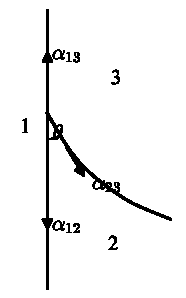
\includegraphics[width=5.5cm]{fig79.pdf}\\[0.3em]{\small 图 79}\end{minipage}\par\nopagebreak

如果 $\alpha_{13}>\alpha_{12}$，亦即气体和固体之间的表面张力大于固体和液体之间的表面张力，那么 $\cos\theta>0$，因而接触角是锐角（如图79所示）.如果 $\alpha_{13}<\alpha_{12}$，那么接触角是钝角.

由(161.1)式可以看出：稳定接触的任何实际情况，应当满足不等式
\begin{equation}
  |\alpha_{13}-\alpha_{12}|\leqslant\alpha_{23};
\end{equation}
否则平衡条件会导致无意义的虚值角度 $\theta$.另一方面，如果我们把 $\alpha_{12},\alpha_{13},\alpha_{23}$ 理解为一对物体在没有第三者时自身相应的表面张力系数值，那么条件(161.2)完全有可能不满足.但是实际上应当注意到：当三种不同的物质相互接触时，在它们每两种的界面上，一般有可能形成第三种物质的吸附膜，而降低表面张力.结果所得到的系数 $\alpha$ 总是满足不等式(161.2)，而这样的吸附一定会发生，否则这个不等式就不被满足.

如果液体完全润湿固体表面，那么在固体表面上所形成的不是吸附膜，而是宏观厚度的液膜.结果，气体将到处与同一液体接触，而固体和气体之间的表面张力根本不用考虑.力学平衡条件直接给出 $\cos\theta=1$，即接触角等于零.

如果相互接触的三个物体中没有一个是固体，而是一个液滴（图80中的3）在另一种液体(1)的表面上，而后者又与气体(2)邻接，则可作类似讨论.在这种情形下，接触角 $\theta_1$ 和 $\theta_2$ 由三个表面张力的合力为零来决定，即矢量和
\begin{equation}
  \alpha_{12}+\alpha_{13}+\alpha_{23}=0.
\end{equation}
显然，这时 $\alpha_{12},\alpha_{13},\alpha_{23}$ 中每一个量的大小应当不大于另两个之和，而不小于它们之差.

\par\nopagebreak\noindent\begin{minipage}{\linewidth}\centering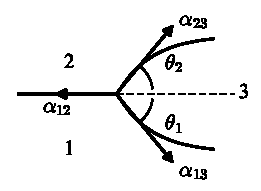
\includegraphics[width=5.5cm]{fig80.pdf}\\[0.3em]{\small 图 80}\end{minipage}\par\nopagebreak

\section{相变时的成核}

如果一种物质处于亚稳态，那么它迟早会进入另一个呈稳定的状态.例如，过冷的蒸气终究会凝聚成为液体；过热的液体会转变成为蒸气.这种相变以下述方式发生.在均匀相中，由于涨落的缘故，会形成小团的另一相；例如，在蒸气中形成小液滴.如果蒸气是稳定相，那么这些小液滴总是不稳定，终究消失.但是如果蒸气是过冷的，那么其中出现的小液滴足够大时，会随时间继续生长，而充当蒸气的凝聚中心.小液滴必须具备足够的大小，才能补偿在液体和蒸气之间出现界面所引起的能量上的不利效应\footnote{必须注意，这里所描述的形成新相的机理，只有在足够纯的物质中才能真正实现.实际上，形成新相中心的通常是各种类型的“杂质”如尘土、离子.}.

因此，存在一个特定的最小临界尺度，亚稳相中生成的新相的所谓核应该具备这样的尺度，才能成为形成新相的中心.因为究竟哪一相稳定，取决小于还是大于临界的尺度，所以“临界核”同亚稳相处于不稳定平衡.下面将讨论出现这种核的概率\footnote{关于任意大小核的出现概率的计算，及所述关系式的说明，参看习题2.}.相变的起点取决于正好具有最小必要尺度的核的出现概率（详见第10卷）.

我们考虑在各向同性相中核的形成：在过冷蒸气中形成液滴，或者在过热的液体中形成蒸气泡.核可以认为是球形，因为它的尺度很小，重力对它形状的影响完全可略.对于同周围介质处于平衡的核，根据(156.2)有
\begin{equation*}
  P'-P=\frac{2\alpha}{r},
\end{equation*}
由此得出核的半径为
\begin{equation}
  r_c=\frac{2\alpha}{P'-P}
\end{equation}
（凡带撇量属于核，不带撇量则属于基本的亚稳相）.

根据普遍公式(112.1)，涨落生成核的概率 w 正比于 $\exp\left(-R_{\mathrm{min}}/T\right)$，式中 $R_{\mathrm{min}}$ 是形成该核所需的最小功.因为核的温度和化学势与周围介质（基本相）有相同值，所以这个功等于该过程中热力学势 $\Omega$ 的变化.核形成以前，亚稳相的体积等于 $V+V'$，而它的热力学势为 $\Omega=-P(V+V')$. 体积 $V'$ 的核形成以后，整个系统的热力学势为 $\Omega=-PV-P'V'+\alpha\mathfrak{s}$. 所以，
\begin{equation}
  R_{\mathrm{min}}=-(P'-P)V'+\alpha\mathfrak{s}.
\end{equation}
对于球形核 $V'=\dfrac{4}{3}\pi r^3,\ \mathfrak{s}=4\pi r^2$，并用(162.1)来表示 r，我们求得
\begin{equation}
  R_{\mathrm{min}}=\frac{16\pi\alpha^3}{3(P'-P)^2}.
\end{equation}
正像在§156中一样，当两相之间的分界为平面时，我们用符号 $P_0$ 表示两相（在给定温度 T 下）的压强；换句话说，压强取值 $P_0$ 时，给定的温度 T 是通常的相变点，过热或者过冷都相对它而言.如果亚稳相仅仅稍为过热或者过冷，则差 $\delta P=P-P_0,\ \delta P'=P'-P_0$ 都相对较小，并且由关系式(156.4)相联系：
\begin{equation}
  v'\delta P'=v\delta P,
\end{equation}
式中 $v'$ 和 v 为核和亚稳相的分子体积.在公式(162.3)中用 $\delta P'-\delta P$ 取代 $P'-P$ 并且由(162.4)用 $\delta P$ 表示 $\delta P'$，可得在稍为过热或过冷的相中形成一个核的概率：
\begin{equation}
  w\propto\exp\left\{-\frac{16\pi\alpha^3v'^2}
  {3T(v-v')^2(\delta P)^2}\right\}.
\end{equation}
如果考虑在过热液体中形成蒸气泡，则在该公式中 v 与 $v'$ 相比可略，于是
\begin{equation}
  w\propto\exp\left\{-\frac{16\pi\alpha^3}{3T(\delta P)^2}\right\}.
\end{equation}
至于在过冷蒸气中形成液滴，在(162.5)中 $v'$ 与 v 相比可略，而对于 v 可以用 $v=T/P\approx T/P_0$ 代入. 这就给出
\begin{equation}
  w\propto\exp\left\{-\frac{16\pi\alpha^3v'^2P_0^2}
  {3T^3(\delta P)^2}\right\}.
\end{equation}
亚稳定性的程度可以用差 $\delta T=T-T_0$ 代替 $\delta P$ 来度量，这里 T 是亚稳相（核与之处于平衡）的温度，$T_0$ 是界面为平面时两相平衡的温度.根据克拉珀龙-克劳修斯公式，$\delta T$ 和 $\delta P$ 由下式相联系：
\begin{equation*}
  \delta P=\frac{q}{T_0(v-v')}\,\delta T,
\end{equation*}
式中 q 是从亚稳相到核所在相的分子相变潜热.把这个式子代入(162.5)，可得形成核的概率
\begin{equation}
  w\propto\exp\left\{-\frac{16\pi\alpha^3v'^2T_0}
  {3q^2(\delta T)^2}\right\}.
\end{equation}
如果饱和蒸气同固体表面（器壁）接触，而后者又能够被该种液体完全润湿，则蒸气的凝聚就直接发生在这个固体表面上，而不形成任何核.在这种情况下，在固体表面上形成液膜不需要做功去形成表面，因而亚稳相（过冷蒸气）不可能存在.

由于同样的原因，表面暴露的固体一般来讲也不可能过热，因为液体通常能完全湿润同种物质的固相表面，而这意味着：在熔化物体的表面形成液层不需要做功去形成新表面.

然而，在熔化中的晶体内部形成核仍有可能，只要保持适当的加热条件：物体从内部加热，并且它的表面温度保持在熔点以下.这种核的形成概率主要依赖于固体中与形成液滴相伴的弹性形变.

\begin{xiti}

\noindent{\heiti 习题1}\quad 试求液体在固体表面上成核的概率，假定接触角的值已知为 $\theta$（非零）.

解：液态核具有球缺的形状，其底的半径为 $r\sin\theta$（r 为相应球体的半径）.它的体积等于
\begin{equation*}
  V=\frac{\pi r^3}{3}(1-\cos\theta)^2(2+\cos\theta),
\end{equation*}
它的球面部分面积和底面积各为 $2\pi r^2(1-\cos\theta)$ 和 $\pi r^2\sin^2\theta$. 利用确定接触角的关系式(161.1)，可以求出核形成时 $\Omega_s$ 的改变等于
\begin{equation*}
  \alpha\cdot2\pi r^2(1-\cos\theta)-\alpha\cos\theta\cdot\pi r^2\sin^2\theta
  =\alpha\pi r^2(1-\cos\theta)^2(2+\cos\theta),
\end{equation*}
式中 $\alpha$ 是在液体和蒸气的界面上的表面张力系数.$\Omega_s$ 的这一改变相当于在蒸气中形成一个体积为 V 的液态核，且其表面张力为
\begin{equation*}
  \alpha_{\mathrm{eff}}=\alpha\left(\frac{1-\cos\theta}{2}\right)^{2/3}
  (2+\cos\theta)^{1/3}.
\end{equation*}
相应地，在正文导得的成核概率公式中用 $\alpha_{\mathrm{eff}}$ 代替 $\alpha$，我们就得到所求的公式.

\noindent{\heiti 习题2}\quad 求任意大小的核形成时的 $R_{\mathrm{min}}$.

解：把亚稳相看成外部介质，核在其中；计算成核所做的功可采用公式(20.2)：$R_{\mathrm{min}}=\Delta(E-T_0S+P_0V)$，考虑到这里该过程温度不变，就发生在介质的温度下，所以 $R_{\mathrm{min}}=\Delta(F+P_0V)$. 这个量的确定，只需考虑转变成另一相的物质量（因为在亚稳相中的其余大量物质的状态保持不变）.仍用不带撇和带撇的字母分别表示原始相和新相中的量，有
\begin{equation*}
\begin{aligned}
  R_{\mathrm{min}}&=\left[F'(P')+PV'+\alpha\mathfrak{s}\right]
  -\left[F(P)+PV\right]=\\
  &=\Phi'(P')-\Phi(P)-(P'-P)V'+\alpha\mathfrak{s};
\end{aligned}
\tag{1}
\end{equation*}
如果核与亚稳相处于不稳定平衡，则 $\Phi'(P')=\Phi(P)$，又回到(162.2).

假定亚稳定度很小，有 $\Phi'(P')\approx\Phi'(P)+(P'-P)V'$，因此(1)化为 $R_{\mathrm{min}}=n[\mu'(P)-\mu(P)]+\alpha\mathfrak{s}$，式中 $n=V'/v'$ 是核中的粒子数.对于球形核
\begin{equation*}
  R_{\mathrm{min}}=-\frac{4\pi r^3}{3v'}\left[\mu(P)-\mu'(P)\right]
  +4\pi r^2\alpha.
\tag{2}
\end{equation*}
在亚稳区，$\mu(P)>\mu'(P)$，因此第一项（体积项）是负的.可以说，表达式(2)描述了在形成稳定核时应克服的势垒.在相当于核临界尺寸的 r 值处：
\begin{equation*}
  r=r_c=\frac{2\alpha v'}{\mu(P)-\mu'(P)},
\end{equation*}
它有极大值.当 $r<r_c$ 时，减小 r 在能量上有利而核消解；当 $r>r_c$ 时，增加 r 有利而核生长\footnote{如果注意到在 $r=r_c$ 的条件下 $\mu(P)-\mu'(P)\approx(v-v')\delta P$，这时计算 $R_{\min}$ 当然导致在正文中得到的公式(162.5).这里指出，对于 $r>r_c$，概率公式(112.1)没有意义，因为存在这种核时介质不稳定.}.

\end{xiti}

\section{相在一维系统中存在的不可能性}

在一维（线型）系统（即粒子置于一条线附近的系统）中是否可能有不同的相存在，这是一个具有理论意义的问题.下面的讨论能够对这个问题给出一个否定的回答：相互接触在一点且具有任意大尺度即长度的两个均匀相之间，不可能有热力学平衡（Л. Д. Ландау, 1950）.

为了证明这个论断，我们设想一个线型系统由两相的线段交替连接而成.设 $\Phi_0$ 是这个系统在不考虑两相间有接触点存在时的热力学势；换句话说，它是两相热力学势的总量，而与如何划分成段无关.为了考虑上述接触点的影响，我们可以把这个系统形式地看作这些点在两相中的“溶液”.如果这个“溶液”是稀的，那么系统的热力学势 $\Phi$ 具有形式
\begin{equation*}
  \Phi=\Phi_0+nT\ln\frac{n}{\mathrm{e}L}+n\psi,
\end{equation*}
其中 n 是长度 L 中的接触点数.因此
\begin{equation*}
  \frac{\partial\Phi}{\partial n}=T\ln\frac{n}{L}+\psi.
\end{equation*}
在足够小的“浓度”$\dfrac{n}{L}$ 下（即两相的线段数目不多），$\ln\dfrac{n}{L}$ 是负的且绝对值很大，以致
\begin{equation*}
  \frac{\partial\Phi}{\partial n}<0.
\end{equation*}
由此可见，$\Phi$ 随着 n 的增大而减小，而因为 $\Phi$ 应当趋于极小值，所以这意味着 n 会增大（直到微商 $\dfrac{\partial\Phi}{\partial n}$ 变正）.换句话说，两相有变成愈来愈小的线段而混合的趋势，也就是说，根本不可能作为分离的两相而存在.

但是，我们指出，$\partial\Phi/\partial n$ 的表达式中的对数主导项正比于温度.因此所述的结论不适用于绝对零度温度.
